\documentclass[uplatex]{jsarticle}
\usepackage[dvipdfmx]{graphicx}
\usepackage{ascmac}
\usepackage{listings}
\usepackage{amsmath}
\usepackage{bm}
\usepackage{cases}

\DeclareMathOperator*{\minimize}{minimize}


\title{人工知能 課題番号1「人工知能の実現可能性について考察せよ」}
\author{工学部電子情報工学科 03-175001 浅井明里}

\makeatletter
\def\maketitle{%
  \null
  \thispagestyle{empty}%
  \vfill
  \begin{center}\leavevmode
    \normalfont
    {\LARGE \@title\par}%
    \vskip 1cm
    {\Large \@author\par}%
    \vskip 1cm
    {\Large \@date\par}%
  \end{center}%
  \vfill
  \null
  \@thanks%\vfil\null
  \cleardoublepage
  }
\makeatother


\title{人工知能 課題番号25「多目的PCOの実装」}
\author{工学部電子情報工学科 03-175001 浅井明里}
\date{\today}

\begin{document}
\maketitle

% \section{モンテカルロ探索法とは}
% \subsection{モンテカルロ探索法と従来の手法との相違点}

\section{本課題について}
本課題では、個体群に基づく最適化アルゴリズムの一つである粒子群最適化アルゴリズム
(Particle Swarm Optimizers、以下PCO)をpythonで実装し、
それを多目的関数最適化を可能にするよう拡張、
また結果を3次元プロットにより可視化した。

\section{PSOアルゴリズム及びMOPSOアルゴリズムについて}
PSOは探索の対象となる目的関数が与えられたとき、
複数の粒子が互いに情報を共有しながら最適解を求めて探索空間内を動き回ることにより
最適化を行うアルゴリズムである。柔軟な並列処理が可能であること、
勾配情報を用いない探索が可能であること、
また非線形システムにも対応が可能なことなど様々な利点があり、
画像処理や組合せ最適化、ゲーム戦略など、様々な領域に応用が可能である。

まず、PSOの基本アルゴリズムについて説明を行う。
$M$次元の探索空間$S_0$で、正定関数$F$の最小値を探索することで考える。
$$F_x \leq C_1,\ {\bf x} = (x_1, \ldots , x_M) \in S_0$$
これはある閾値$C_1$以下となる${\bf x}$を探索する。
$C_1 = 0$が厳密値の探索であり、$0 < C_1$が近似解の探索に対応する。
PSOでは$N$個の粒子が探索空間$S_0$を動き回って解を探索する。各粒子は
$$位置\ :\ x^i = (x_1^i, \ldots, x_M^i),\ 速度\ :\ v^i = (v_1^i, \ldots, v_M^i)$$
により特徴付けられる。ここで$i$はそれぞれの粒子につけられたID(インデクス)である。各粒子は
$S_0$内に与えられた初期位置から与えられた初期速度で動作を開始する。この動作においては、以下の二つの
量が重要となる。

\begin{description}
  \item[パーソナルベスト]\mbox{}\\
  $i$番目の粒子の現在までの最良値を与える粒子位置。$p^i = (p_1^i, \dots p_N^i)$ \\
  また、全ての粒子のパーソナルベストの最良値をグローバルベスト$g = (g_1, \ldots, g_N)$
  と呼ぶ。
  \item[ローカルベスト]\mbox{}\\
  $i$番目の粒子の近傍のパーソナルベストの最良値。$l^i = (l_1^i, \dots l_N^i)$\\
  ここで近傍は粒子の結合形態に依存して決まる。
  全結合を仮定するとき、ローカルベストとグローバルベストは一致する。各粒子の相互作用は
  目的関数に基づくローカルベストを介してなされ、その相互作用によって、粒子群が形成される。

  今回の実装にあたっては、粒子の更新式は以下のものを用いた。
  $$v_j^i(n+1) = wv_j^i(n) + \alpha_1(p_j^i - x_j^i(n)) + \alpha_2(l_j^i - x_j^i(n))$$
  $$x_j^i(n+1) = x_j^i(n) + v_j^i(n)$$
  ここで$w, \alpha_1, \alpha_2$はパラメータである。
  パーソナルベストは各時刻の目的関数の値によって更新される。
  $$p_i = x^i(n)\ {\rm if}\ Fx^i(n)) < F(p^i)$$
  またこのパーソナルベストの更新と連動して、ローカルベストとグローバルベストを更新する。
\end{description}

\section{Multi-Objective PSOの実装}
今回はこのPSOアルゴリズムを多目的関数に対応できるよう拡張したMulti-Objective Particle Swarm Optimizationを実装した。
Kumar and Minz(2014)はMulti-Objective Particle Swarm Optimizationを実装する方法をいくつかあげているが、
今回はそのうち最も広く用いられていると言われている、重み付けされた目的関数を複合し、一つの目的関数に置き換える方法を採用した。

目的関数の重み付け和は以下の式で表される。
$$F(x) = \sum_{i=1}^k w_i f_i(x)$$
ここで$i=1,2,3, \ldots, k$はk個の目的関数に与えられた
インデクスであり、重みは全体で1になる非負の数である。
$$\sum_{i=1}^k w_j = 1$$
この関数の重み付けを動的に変更するアルゴリズムにBang-Bang
Weighted Aggregation(BWA)とDynamic Weighted Aggregation(DWA)
があり、今回はDWAを利用した。
DWAは二つの目的関数に対する重み付けを以下の式に従って動的に変更する。
$$w_1(t) = \left|\sin{\left(\frac{2\pi t}{f_w}\right)}\right|$$
$$w_2(t) = 1 - w_1(t)$$

\section{実装及び結果}
Multi-Objective Particle Swarm Optimizationについてはmopso.pyという
ファイルにて、MOPSOクラスが定義されており、
また同ファイル内のvisualize\_result()関数によってcsvファイルに保存された粒子の位置が
三次元上にプロットできる。

MOPSOクラスについてはx及びyの最大最小値などを渡して初期化をしたのち、
任意の関数を定義しこの関数オブジェクトをset\_objective\_functions関数に渡すことで、
あるMOPSOインスタンスの目的関数に指定できる。実際に粒子の位置及び速度を更新するのは
update\_particles関数であり、これを指定されたステップ数実行し終わることを終了条件としている。

今回は以下の$f_1, f_2$を目的関数としてMOPSOによりより良い解の探索を行った。
$$f_1 = x^2 + y^2$$
$$f_2 = \sin{(x)} + \cos{(y)}$$
この結果をプロットしたものが次の図1であり、
実際に$f_1及びf_2$が小さくなるような$(x,y)$周辺に粒子が集まっている様子が確認できる。
\begin{figure}
  \begin{center}
    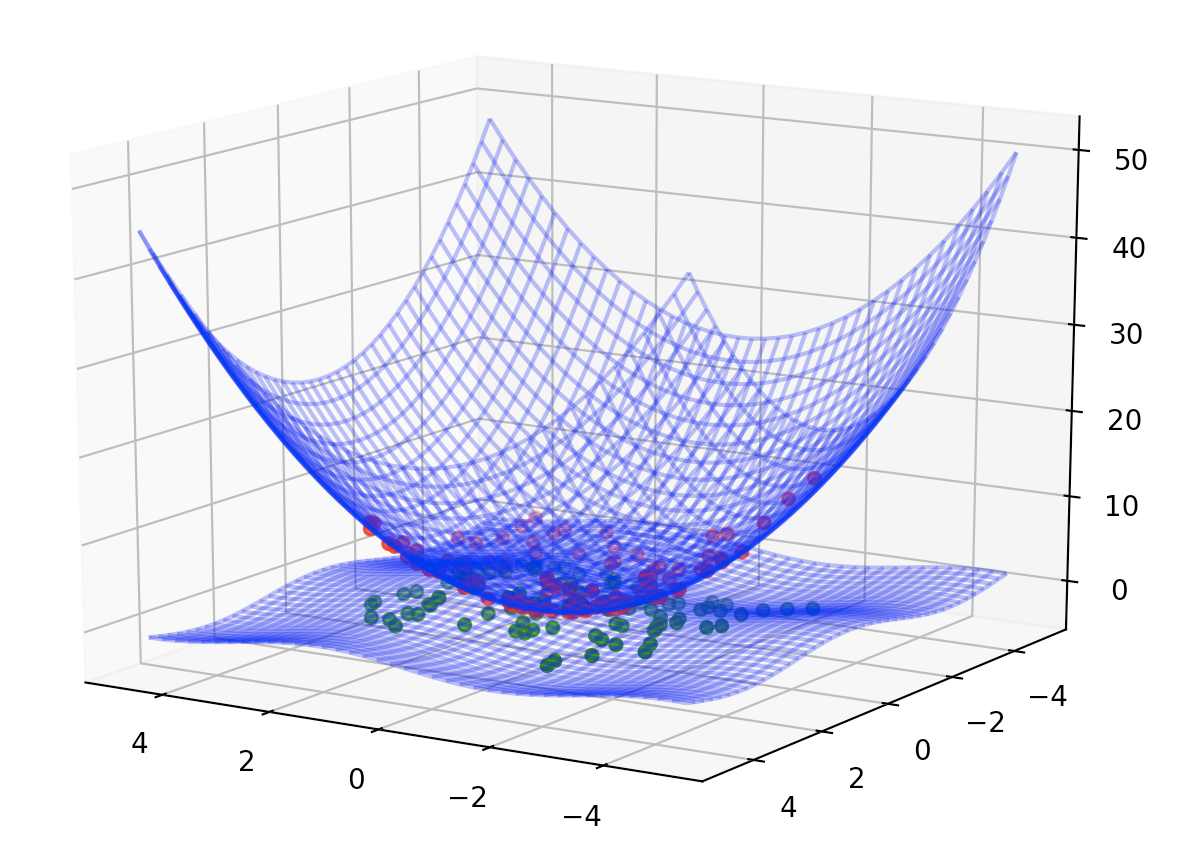
\includegraphics[width=15cm]{mopso_result.png}
    \caption{MOPSOアルゴリズム結果の三次元プロット}
  \end{center}
\end{figure}

\begin{thebibliography}{9}
\bibitem{sinsuphan} Vipin Kumar and Sonajharia Minz, "Multi-Objective Particle Swarm Optimization: An Introduction", Smart Computing Review, vol.4,
no.5, p.335-353. 2014.
\bibitem{sinsuphan}斎藤利道『粒子群最適化と非線形システム』電子情報通信学会 基礎・境界ソサイエティ Fundamentals Review 5巻2号. p.155-161. 2011.
\end{thebibliography}







\end{document}
